\documentclass[a4paper,12pt]{article}
\usepackage{setspace}
\usepackage{sectsty}
\usepackage{siunitx}
\usepackage{graphicx}
\usepackage[a4paper, total={3in, 9in}, textwidth=16cm,bottom=1in,top=1.4in]{geometry}
\usepackage[dvipsnames]{xcolor}
\usepackage{amsmath}
\usepackage{esvect}
\usepackage{soul}
\usepackage{amsthm}
\usepackage{hyperref}
\usepackage{float}
\usepackage{amssymb}
\usepackage{outlines}
\usepackage{caption}
\usepackage{fancyvrb}
\usepackage{subcaption}
\usepackage{esdiff}
\usepackage{colortbl}
\usepackage{booktabs}
\usepackage{setspace}
\usepackage{mathtools}
\usepackage{tikz,pgfplots}
\usepackage[most]{tcolorbox}
\usepackage{draftwatermark}
\SetWatermarkText{timthedev07}
\SetWatermarkScale{4}
\SetWatermarkColor[gray]{0.97}
\usetikzlibrary{positioning,decorations.markings,arrows.meta}
\DeclarePairedDelimiter{\ceil}{\lceil}{\rceil}
\newtheorem{lemma}{Lemma}
\newtheorem{proposition}{Proposition}
\newtheorem{remark}{Remark}
\newtheorem{observation}{Observation}
\doublespacing
\let\oldsection\section
\renewcommand\section{\clearpage\oldsection}
\newcommand{\RNum}[1]{\uppercase\expandafter{\romannumeral #1\relax}}
\let\oldsi\si
\renewcommand{\si}[1]{\oldsi[per-mode=reciprocal-positive-first]{#1}}
\usepackage{enumitem}
\newcommand{\subtitle}[1]{%
  \posttitle{%
    \par\end{center}
    \begin{center}\large#1\end{center}
    \vskip0.5em}%
}
\newcommand{\degsym}{^{\circ}}
\newcommand{\Mod}[1]{\ (\mathrm{mod}\ #1)}
\usepackage{hyperref}
\hypersetup{
  colorlinks=true,
  linkcolor = blue
}
\newcommand{\lb}{\\[8pt]}
\newenvironment*{cell}[1][]{\begin{tabular}[c]{@{}c@{}}}{\end{tabular}}
\newcommand{\img}[4]{\begin{center}
  \begin{figure}[H]
    \centering
    \includegraphics[width=#2\textwidth]{#1}
    \caption{#3}
    \label{fig:#4}
  \end{figure}
\end{center}}
\parindent=0pt
\usepackage{fancyhdr}
\fancyfoot{}
\fancypagestyle{fancy}{\fancyfoot[R]{\vspace*{1.5\baselineskip}\thepage}}
\renewcommand{\contentsname}{Table of Contents}
\newcommand{\angled}[1]{\langle{#1}\rangle}
\newcommand{\paren}[1]{\left(#1\right)}
\newcommand{\sqb}[1]{\left[#1\right]}
\newcommand{\coord}[3]{\angled{#1,\, #2,\, #3}}
\newcommand{\pair}[2]{\paren{#1,\, #2}}
\newcommand{\atom}[3]{{}^{#1}_{#2}\text{#3}}
\usepackage[
  noabbrev,
  capitalise,
  nameinlink,
]{cleveref}

\crefname{lemma}{Lemma}{Lemmas}
\crefname{proposition}{Proposition}{Propositions}
\crefname{remark}{Remark}{Remarks}
\crefname{observation}{Observation}{Observations}

\newtcolorbox[auto counter]{prob}[2][]{fonttitle=\bfseries, title=\strut Problem~\thetcbcounter: #2,#1,colback=Orchid!5!white,colframe=Orchid!75!black,top=5mm,bottom=5mm}

\newtcolorbox[auto counter]{rem}[1][]{fonttitle=\bfseries, title=\strut Remark.~\thetcbcounter,colback=purple!5!white,colframe=purple!65!gray,top=5mm,bottom=5mm}

\newtcolorbox[auto counter]{defin}[1][]{fonttitle=\bfseries, title=\strut Definition.~\thetcbcounter,colback=black!5!white,colframe=black!65!gray,top=5mm,bottom=5mm}

\newtcolorbox[auto counter]{obs}[1][]{fonttitle=\bfseries, title=\strut Observation.~\thetcbcounter,colback=RedViolet!5!white,colframe=RedViolet!65!gray,top=5mm,bottom=5mm}

\newtcolorbox[auto counter]{lem}[1][]{fonttitle=\bfseries, title=\strut Lemma.~\thetcbcounter,colback=Maroon!5!white,colframe=Maroon!65!gray,top=5mm,bottom=5mm}

\newtcolorbox[auto counter]{prop}[1][]{fonttitle=\bfseries, title=\strut Proposition.~\thetcbcounter,colback=RedOrange!5!white,colframe=RedOrange!65!gray,top=5mm,bottom=5mm}

\newtcolorbox[auto counter]{hint}[1][]{fonttitle=\bfseries, title=\strut Hint.~\thetcbcounter,colback=OliveGreen!5!white,colframe=OliveGreen!75!gray,top=5mm,bottom=5mm}

\setlength{\belowcaptionskip}{-20pt}
\begin{document}


\pagenumbering{arabic}
\pagestyle{fancy}


\begin{titlepage}
  \begin{center}

    \vspace*{8cm}
    \textbf{\Large {IB Physics Topic E3 Radioactive Decay; SL \& HL}} \\
    \vspace*{1cm}
    \large{By timthedev07, M25 Cohort}

  \end{center}
\end{titlepage}

\pagebreak
\tableofcontents
\pagebreak

\clearpage
\setcounter{page}{1}
\addtocontents{toc}{\protect\thispagestyle{empty}}

\section{Isotopes and Isotones}

Definitions:

\begin{itemize}
  \item Isotopes are a set of atoms that have the same proton number but different nucleon numbers; i.e. they have different numbers of neutrons. They possess the same chemical properties but different physical properties.
  \item Isotones are a set of atoms with the same number of neutrons but different numbers of protons \& electrons.
  \item A nuclide is a distinct kind of atom or nucleus characterized by a specific number of protons and neutrons. E.g. carbon-12 is a nuclide of carbon with 6 protons and 6 neutrons.
\end{itemize}

\section{Radioactive Decay}

It is a random and natural process that happens to any unstable nucleus (iterative process until stability). Before the decay, the nucleus is referred to as the \textbf{parent nuclide}, and after the decay, the nucleus is referred to as the \textbf{daughter nuclide}. The sequence of decays is referred to as a \textbf{radioactive series} or \textbf{decay chain}.\lb
Radioactive decay has the below properties
\begin{itemize}
  \item Arbitrary
  \item Spontaneous --- one cannot influence the rate of decay by changing physical conditions of the sample such as its temperature, pressure, etc. This is not to be confused with fusion and fission.
\end{itemize}

For any radioactive decay to take place, the \textbf{difference in energy} between parent and daughter nuclides must be \textbf{sufficiently large}.

\pagebreak

\subsection{Types of Decay}

\subsubsection{Alpha Decay}

Alpha decay is the process where an unstable nucleus emits an alpha particle (\textbf{two protons, two neutrons}, $^4_2\text{He}$), reducing both atomic number $Z$ and mass number $A$:
\[
  \atom{A}{Z}{X} \rightarrow \atom{A-4}{Z-2}{Y} + \atom{4}{2}{He}
\]

For example, uranium-238 decays as:

\[
  \atom{238}{92}{U} \rightarrow \atom{234}{90}{Th} + \atom{4}{2}{He}
\]

Most of the released energy is transferred to the alpha particle due to its smaller mass.

Momentum is conserved in the system. The momentum of the daughter nucleus and the alpha particle must be equal and opposite:

\[
  M_{\text{daughter}} v_{\text{daughter}} = - M_{\alpha} v_{\alpha}
\]

Because $M_{\text{daughter}} \gg M_{\alpha}$, the alpha particle moves much faster.

They are highly ionizing but \textbf{lose energy quickly}, making them easily stopped by paper or a few centimeters of air. All alpha particles emitted by the same decay event have the \textbf{same initial energy}, and they lose \textbf{roughly a fixed amount of energy per collision} with each air atom as they travel.
The \textbf{mass ratio} of the alpha particle and the daughter/parent nucleus can be accurately estimated by the \textbf{ratio of their nucleon numbers}.
They are more ionizing than gamma photons because they are \hl{electrically charged and hence more likely to interact with electrons in the surrounding material}. They are also more ionizing than beta particles because they are \hl{heavier and slower} and \hl{carry a larger charge}.

\pagebreak

\subsubsection{Beta Decay}

\begin{itemize}
  \item \textbf{Beta-minus decay} is the process where a neutron decays into a proton, an electron, and an antineutrino. The \textbf{electron is emitted} from the nucleus, the \textbf{proton is retained} within the nucleus, and \textbf{the antineutrino (an antiparticle, signified by the overbar) is emitted to conserve momentum}. This occurs to atoms whose $\dfrac{\text{neutron}}{\text{proton}}$ ratio is too high, e.g. $^{132}_{52}$Te, which has 80 neutrons and 52 protons.
        \[
          \atom{A}{Z}{X} \rightarrow \atom{A}{Z+1}{Y} + e^- + \bar{\nu}_e
        \]
        This occurs when the neutron-to-proton ratio is too high, in which case, it is desired to increase the proton number by losing an electron.

        Antineutrinos have no effective mass or charge.

        The momentum equation in this case does not have a single solution, as there are three emitted particles.
  \item \textbf{Beta-plus decay} is the process where a proton decays into a neutron, a positron, and a neutrino:
        \[
          \atom{A}{Z}{X} \rightarrow \atom{A}{Z-1}{Y} + e^+ + \nu_e
        \]
  \item \textbf{Electron capture} is the process where an electron on the \textbf{inner shell} is captured by the nucleus, converting a proton into a neutron and releasing a neutrino. This is another way to increase the neutron-to-proton ratio. The energy difference between the parent and daughter nuclides is small, and so a positron cannot be created.
        \[
          \atom{A}{Z}{X} + e^- \rightarrow \atom{A}{Z-1}{Y} + \nu_e
        \]
\end{itemize}

An alternative notation for $e^+$ is $\atom{0}{-1}{$\beta$}$, and for $e^-$ is $\atom{0}{+1}{$\beta$}$.

\pagebreak

\subsubsection{Gamma Decay}

\begin{itemize}
  \item Gamma decay is the process where an unstable nucleus emits a gamma ray.
  \item A gamma ray is a high-energy photon, its energy level is usually measured in MeV. The energy of the gamma ray is equal to the energy difference between the parent and daughter nuclides. The atomic and mass numbers remain the same.
  \item Can be a subsequent decay after alpha or beta decay, when the daughter nucleus is in an excited state with a surplus of energy.
  \item Evidence for quantized \textbf{nuclear energy levels}.
\end{itemize}

\subsection{Energy Levels}

\subsubsection{Discrete Energy Levels}

This holds true for energy changes in \textbf{gamma} and \textbf{alpha} decay, because the former is simply an emission of photons and the latter is simply an emission of a helium nucleus.

\subsubsection{Continuous Energy Levels}

\textbf{In beta decay}, the total decay energy is fixed, but it must be shared between the daughter nuclide, the emitted electron/positron, and the neutrino/antineutrino. The sharing of energy is not discrete but \textbf{continuous}.
\begin{itemize}
  \item Momentum and energy are still conserved, but in a three body decay, there is no unique solution for the momentum of the daughter nucleus, the emitted electron, and the neutrino.
  \item The shape of the spectrum shows that there are more beta particles with lower energies, and fewer particles near the maximum energy.
  \item The energy spectrum is described by a probabilistic function that accounts for the interaction between the beta particle and the nucleus.
\end{itemize}

\section{Properties of Ionizing Radiation}

To \textbf{ionize} a material means to remove or add electrons to atoms or molecules within the material, thereby creating ions. When ionizing radiation passes through matter, it can ionize the material, thereby \textbf{transferring energy} from the energetic particle to separate the electron from the ion.
\begin{itemize}
  \item For an alpha/beta particle, the ionization reduces the energy of the particle in a continuous manner.
  \item For a gamma ray, or an emitted photon, the photon is either completely absorbed or will experience a \textbf{frequency shift}, where the frequency drops and wavelength increases.
\end{itemize}
\begin{table}[h!]
  \centering
  \def\arraystretch{2}
  \begin{tabular}{|>{\columncolor{gray!10}}c|c|c|c|}
    \hline
    \rowcolor{blue!30}
    \hline
    \rowcolor{blue!30}
    \textbf{Type} & \textbf{Ionization} & \textbf{Penetration} & \textbf{Range}                                   \\
    \hline
    Alpha         & High                & Low                  & Few cm in air (absorbed by paper)                \\
    \hline
    Beta          & Moderate            & Moderate             & Several m in air (absorbed by mm of plastic)     \\
    \hline
    Gamma         & Low                 & High                 & Hundreds of m in air (absorbed by lead/concrete) \\
    \hline
  \end{tabular}
  \caption{Comparison of Alpha, Beta, and Gamma Radiation}
\end{table}

\section{Mass Defect and Binding Energy}

\textbf{Binding energy} is the energy that holds the nucleus together. It is also the \textbf{required amount of energy to separate the nucleus} into its constituent protons and neutrons. The excess of energy, above the level of the binding energy, that is supplied to the nucleus, will be converted to the kinetic energy of the emitted particles.\lb
Moreover, when a neutron and a proton collide and combine to form a deuteron, they release energy, in the form of a photon, also at the level of binding energy as they form the bound.\lb
When protons and neutrons (collectively, nucleons) combine to form an atomic nucleus, the total mass of the nucleus is slightly less than the sum of the individual masses of the protons and neutrons. This difference in mass is called the \textbf{mass defect}. It arises because some of the mass of the nucleons is converted into energy \textbf{to bind the nucleus together}; there is a mass defect in \textbf{both fusion and fission}. The formalized relation is given by
$$E = \Delta mc^2$$
\begin{itemize}
  \item $E$ is the energy released when the nucleus is formed; binding energy
  \item $\Delta m$ is the mass defect.
  \item $c$ is the speed of light.
\end{itemize}
Mass defect is also the \textbf{difference} between the mass of the nucleus and the sum of the masses of the protons and neutrons that make up the nucleus.
\begin{align*}
  \text{Mass defect} & = \text{Mass of protons and neutrons} - \text{Mass of nucleus}             \\
  \Delta m           & = \left(Zm_\text{proton} + (A-Z)m_\text{neutron}\right) - M_\text{nucleus}
\end{align*}

\pagebreak

\subsection{Example Question --- Energy Released}

The following data is available for atomic masses for the fusion reaction
$$\atom{2}{1}{H} + \atom{3}{1}{H} \rightarrow \atom{4}{2}{He} + n$$
\begin{table}[H]
  \centering
  \begin{tabular}{|c|c|}
    \hline
    Atom              & Mass (u) \\ \hline
    $\atom{2}{1}{H}$  & 2.0141   \\ \hline
    $\atom{3}{1}{H}$  & 3.0160   \\ \hline
    $\atom{4}{2}{He}$ & 4.0026   \\ \hline
  \end{tabular}
\end{table}
(i) Show that the energy released is about 18 MeV.
\begin{align*}
  \mu = \text{Mass defect} & = m_\text{LHS} - m_\text{RHS}                                                        \\
                           & = (2.0141 + 3.0160) - (4.0026 + \underbrace{1.0087}_{\footnotesize{\text{neutron}}}) \\
                           & = 0.0188u                                                                            \\
  \Delta E                 & = \mu c^2
  \\ & = 0.0188 \times 931.5 \approx 17.512 \si{\mega\electronvolt}
\end{align*}
Note that, in exams, simply multiply the mass defect in $u$ (which is about $\SI{1.66e-27}{\kilo\gram}$) by $931.5$ to get the energy released. This constant encapsulates
\begin{itemize}
  \item The conversion factor between $u$ and kg.
  \item The speed of light squared.
  \item The conversion factor between joules and MeV.
\end{itemize}

\pagebreak

\subsection{Binding Energy per Nucleon}

Binding energy per nucleon is simply the binding energy of the nucleus divided by the number of nucleons in the nucleus. It is a measure of the \textbf{stability} of the nucleus: the higher the binding energy per nucleon, the more energy that is required to separate each nucleon from the nucleus, and the more stable the nucleus is. It is given by
$$\frac{E}{A}$$
where $E$ is the binding energy and $A$ is the number of nucleons in the nucleus.

\img{BE_A plot.png}{0.8}{Binding Energy per Nucleon vs. Mass Number}{BE_A}

Features and key information from the graph:
\begin{enumerate}
  \item At the region around $A = 60$, the binding energy per nucleon is at its maximum, indicating that the nucleus is most stable at this point. This includes elements such as iron.
  \item Beyond this optimal point, it is energetically favorable for the nucleus to split into two smaller nuclei to approach the optimal point from right to left; this process is known as \textbf{fission}.
  \item To approach the optimal point from left to right, the nucleus must combine with another nucleus to form a larger nucleus; this process is known as \textbf{fusion}.
  \item In the region from $A = 1$ to $A = 20$, some elements have a binding energy per nucleon that is much higher (and is thus more stable) compared to atoms of similar mass numbers nearby, e.g. helium-4, carbon-12, and oxygen-16.
\end{enumerate}

\subsection{Example Question}
The rest mass of the helium isotope $\atom{3}{2}{He}$ is $m$. What is the expression for the binding energy per nucleon for $\atom{3}{2}{He}$ in terms of $m$, proton mass $m_p$, and neutron mass $m_n$?
\begin{itemize}
  \item The binding energy is in general given by $E = (Zm_p + (A-Z)m_n - m)c^2$.
  \item In this case, $Z = 2$, $A = 3$, and $E = (2m_p + m_n - m)c^2$.
  \item Then, the binding energy per nucleon is given by $\dfrac{E}{A} = \dfrac{(2m_p + m_n - m)c^2}{3}$.
\end{itemize}

\section{The Nucleus}

\subsection{Nuclear Mass}

The unified atomic mass unit, denoted by $u$, is defined as one twelfth of the mass of a carbon, its value is approximately $$1\mathrm{u} \equiv 1.66 \times 10^{-27} \si{\kilo\gram} \equiv 931.5 \si{\mega\electronvolt\per c^2}$$
with uncertainty of $\pm 5\times 10^{-39} \si{\kilo\gram}$.\lb
The \textbf{neutron} has a mass \textbf{slightly greater} than that of a proton.

\hl{Also note that the value of the unified atomic mass in grams and the value of the Avogadro constant in $\si{\per\mol}$ multiply to give 1}.

\subsection{The Strong Nuclear Force}

This force is short-range and attractive; it has the following properties
\begin{itemize}
  \item It is $10^{38}$ times as strong as the force of gravity.
  \item This range is only between nucleons; usually 5 $\si{\femto\m}$ (femtometers)
  \item Is only between nucleons (protons and neutrons)
\end{itemize}

Previous models that did not involve neutrons in the nuclide were unable to explain the stability of the nucleus --- the repulsive forces between protons would inherently cause the nucleus to disintegrate. Thus, there must be an attractive force in the nucleus too; this is the \textbf{strong nuclear force}.

\subsection{Evidence for Strong Nuclear Forces}

\begin{enumerate}
  \item Previously, one has seen that Rutherford's Scattering Experiment, which relies on Coulomb's Law to explain the electrostatic repulsion between the alpha particles and the nucleus, breaks down when the alpha particles are fired at the nucleus with a high enough initial kinetic energy.
  \item Further investigations into the internal structure of the nucleus came from experiments scattering electrons (which don't feel the strong nuclear force).
        \begin{enumerate}
          \item These experiments showed that electrons could be diffracted by the nucleus, and the \textbf{de Broglie wavelength} of the electrons was used to estimate the nuclear size.
          \item When electron energy increases, the scattering becomes inelastic (energy is lost), revealing that protons and neutrons are composed of smaller particles called quarks.
        \end{enumerate}
  \item Binding Energy and the Strong Force:
        \begin{enumerate}
          \item The binding energy per nucleon (energy that holds protons and neutrons together in the nucleus) is relatively constant for medium-heavy nuclei (around $Z \approx 60$).
          \item As you go to heavier nuclei, like uranium-238, the binding energy per nucleon doesn't change significantly, because the strong force mainly acts on nearby nucleons. This suggests that nucleons deep inside the nucleus are shielded from the full effect of the strong force by those at the surface.
        \end{enumerate}
\end{enumerate}

\section{Nuclear Stability}

\img{stability graph.png}{0.8}{Nuclear Stability}{stability}

\begin{enumerate}
  \item For $N, Z \le 15$, the stability area (in dark red) is roughly on the line $A = N$.
  \item For $N, Z > 15$, the stability area starts to move further above the line $A = N$. This means that a $1:1$ \textbf{neutron-to-proton ratio} no longer suffices to keep larger nuclei stable.
  \item The stability line is a rough linear regression of the data points of stable nuclei.
  \item The further a data point is from the stability line, the more unstable the nucleus is, and the more quickly it will decay. We can predict how a nucleus will decay to approach the stability line by inspecting its position relative to the stability line:
        \begin{enumerate}
          \item If the nucleus is above the stability line, it will undergo \textbf{beta-minus decay} to decrease the number of neutrons and increase the number of protons.
          \item If the nucleus is below the stability line, it will undergo \textbf{beta-plus decay} to increase the number of neutrons and decrease the number of protons.
          \item If $A, Z$ are sufficiently high (beyond $A = 60$), in which case, they have the right neutron-proton ratio but just an excessive amount, they will decay by \textbf{alpha decay} to reduce both quantities simultaneously (this keeps the ratio acceptable) and move closer to the stability line diagonally to the bottom left.
        \end{enumerate}
        The graphical transitions are illustrated as follows

        \begin{minipage}{0.3\textwidth}
          \begin{figure}[H]
            \centering
            
\begin{tikzpicture}[thick, decoration={
                    markings,
                    mark=at position 0.6 with {\arrow[scale=1.8]{>}}}]
              \draw (0, 0) grid (1, 1);
              \draw[postaction={decorate}] (0, 1) -- (1, 0);
            \end{tikzpicture}
            \caption{$\beta^-$ decay}
          \end{figure}
        \end{minipage}%
        \begin{minipage}{0.3\textwidth}
          \begin{figure}[H]
            \centering
            
\begin{tikzpicture}[thick, decoration={
                    markings,
                    mark=at position 0.6 with {\arrow[scale=1.8]{>}}}]
              \draw (0, 0) grid (1, 1);
              \draw[postaction={decorate}] (1, 0) -- (0, 1);
            \end{tikzpicture}
            \caption{$\beta^+$ decay}
          \end{figure}
        \end{minipage}%
        \begin{minipage}{0.3\textwidth}
          \begin{figure}[H]
            \centering
            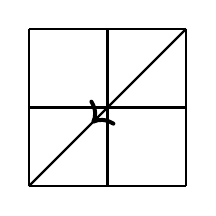
\begin{tikzpicture}[thick, decoration={
                    markings,
                    mark=at position 0.6 with {\arrow[scale=1.8]{>}}}]
              \draw (0, 0) grid (2, 2);
              \draw[postaction={decorate}] (2, 2) -- (0, 0);
            \end{tikzpicture}
            \caption{$\alpha$ decay}
          \end{figure}
        \end{minipage}
\end{enumerate}
It is critical to remember this graph and its characteristics.

\section{Half Lives}

Definitions:
\begin{enumerate}
  \item The \textbf{activity} of a radioactive sample is the number of parent nuclei that decay per unit time. It is measured in becquerels (Bq).
  \item The \textbf{half-life} of a radioactive sample is the time taken for half of the initial sample to decay. It is denoted by $t_{1/2}$.
\end{enumerate}

The decay probability ($\dfrac{1}{2}$) is constant at every stage of the decay chain. The decay behavior obeys the exponential model: Let $N_0$ be the initial activity at time $t = 0$, after $n$ half lives, the remaining activity is given by
$$N' = \frac{N_0}{2^n}$$

\subsection{Idea behind the Exponential Model}

In constant time intervals of size $T$, the ratio $$\frac{\text{number of nuclei that decay between $t = t$ and $t = t + T$}}{\text{number of nuclei at time $t$}}$$
is constant.
Hence, if $A$ is the activity, i.e. the number of decay events per unit time, and $N$ is the initial number of nuclei at the start of the time interval, then \begin{equation}\label{eq:decay_constant}
  A = \lambda N
\end{equation}where $\lambda$ is the \textbf{decay constant} given in $\si{\per\second}$.
By definition, $$A = \diff{N}{t}$$
thus $$\diff{N}{t} = \lambda N$$
we can solve this differential equation to get \begin{equation}\label{eq:NN_0}
  N = N_0 e^{-\lambda t}
\end{equation}
where $N_0$ is the initial number of nuclei at $t = 0$, and $t$ is the time elapsed since then.
We also get an expression for the activity, since $A = \lambda N$
$$A = A_0 e^{-\lambda t}$$
where $A_0 = \lambda N_0$ is the initial activity at $t = 0$. This is a very important equation to remember for this topic.

\subsubsection{Definition of the Decay Constant}

By \cref{eq:decay_constant}, the decay constant can be defined as the \textbf{probability of decay per unit time} for a single nucleus, i.e. $$\lambda = \frac{P}{\Delta t}$$\lb
The claim that the decay probability is the same as the decay constant holds only for tiny time intervals $\Delta t$, compared to the average lifetime of the sample.

\subsubsection{Calculating the Decay Constant}

The decay constant $\lambda$ and the half life $t_{\frac{1}{2}}$ are related by the equation \begin{equation}\label{eq:decay_constant_half_life}
  t_{\frac{1}{2}} = \frac{\ln 2}{\lambda}
\end{equation}

\pagebreak

\subsection{Determining Half Lives}

\subsubsection{Long Half-Lives}

When the half-life of an isotope is too long to be measured, one can combine \cref{eq:decay_constant} and \cref{eq:decay_constant_half_life} to get an estimate for the half-life \begin{equation}\label{eq:long_half_life}
  t_{\frac{1}{2}} = \frac{N\ln 2}{A}
\end{equation}
where the activity $A$ is measured over some manageable time interval.

\subsubsection{Short Half-Lives}

Let $R$ denote the corrected count rate and $R_0$ the initial corrected count rate, by \cref{eq:NN_0}, we can take the natural log of both sides and obtain the following linear equation
$$\ln R = -\lambda t + \ln R_0$$
One can then measure a series of $R$ values and produce a linear graph of $\ln R$ vs. $t$, whose gradient, upon calculation, is $-\lambda$, which can then be substituted into \cref{eq:decay_constant_half_life} to determine the half life.\lb
The advantage of this method is that it works even if $R$ is measured over a period less than the half-life.

\section{Measuring Radioactive Decay}

There are a few devices for measuring radioactive decay:
\begin{enumerate}
  \item The Geiger-Müller Tube: This device measures the number of ionizing particles that pass through it.
        \img{muller.png}{1}{Geiger-Müller Tube}{muller}
        \begin{enumerate}
          \item Structure: Cylindrical chamber filled with low-pressure gas (e.g., argon), with a central anode and outer cathode.
          \item Radiation Detection: Ionizing radiation enters the tube and ionizes the gas, creating \textbf{ion pairs} (free electrons and positive ions).
          \item \textbf{Amplification} of the Signal: Electrons are accelerated by a high voltage field, causing further ionizations in a chain reaction. This allows the reaction to be detected as a signal.
          \item \textbf{Current} Generation: The movement of electrons produces an electric current, detected as a signal for each radiation event.
          \item \textbf{Quenching}: A quenching gas prevents continuous discharge, allowing the tube to reset for subsequent detections. The \textbf{dead time} refers to the time the tube needs to recover from a detection event and be prepared for the next.
        \end{enumerate}
  \item The spark counter
        \begin{enumerate}
          \item Structure: Consists of two metal plates or wires, separated by a small air gap, with a high voltage applied across them.
          \item Working Principle: Detects ionizing radiation by producing visible sparks in the air gap when charged particles pass through.
          \item Ionization Process: When charged particles (alpha or beta particles) enter the air gap, they ionize the air molecules, creating free electrons and positive ions.
          \item Spark Generation: The high voltage accelerates the free electrons, leading to further ionization and creating a discharge (spark) across the gap.
          \item Detection: Each spark corresponds to a charged particle passing through, and the number of sparks indicates the radiation intensity.
        \end{enumerate}
\end{enumerate}

\subsection{Activity and Count Rate}

Definitions:
\begin{enumerate}
  \item The \textbf{activity} of a radioactive sample is the number of parent nuclei that decay per unit time. It is measured in becquerels (Bq).
  \item The \textbf{count rate} is the number of ionizing particles that pass through a detector per unit time. It is measured in counts per second (cps).
\end{enumerate}

The count rate is typically less than and proportional (assuming fixed arrangement) to the actual activity of the sample, because some particles may not be detected by the detector.

\pagebreak

\subsection{Background Radiation}

The background radiation is the ionizing radiation that is always present in the environment, and it comes from various sources:
\begin{itemize}
  \item Radon gas from the ground (a major source): A radioactive gas that seeps into buildings from the ground.
  \item Cosmic radiation: High-energy particles from space that interact with the Earth's atmosphere.
  \item Artificial sources: Medical procedures, nuclear power plants, etc.
  \item Buildings: Building materials like granite contain radioactive elements.
  \item Organisms and consumables: Radioactive isotopes are present in the human body and food.
\end{itemize}

In experiments, to get accurate results, the corrected count rate must be obtained by subtracting the background count rate from the total count rate.

\section{Applications of Radioactive Nuclides}

\subsection{Radioactive Dating}

Determining the age of carbon-based materials by measuring the amount of carbon-14 remaining in the sample. This works for materials up to 60000 years old.
\begin{enumerate}
  \item Plants and organisms absorb carbon-12 and carbon-14 from the atmosphere while alive.
  \item Once dead, the carbon-14 decays to nitrogen-14 while the carbon-12 remains constant. Then, the ratio of carbon-14 to carbon-12 can be used to determine the time elapsed since the organism died.
  \item This works under the assumption that the ratio of carbon-14 to carbon-12 in the atmosphere has remained constant over time while the organism was alive.
\end{enumerate}

\subsection{In Medicine}

In imaging and diagnosis, radioactive isotopes are inhaled, ingested, or injected into the body to trace the movement of substances in the body or emit radiation that can be detected by a special camera.

\begin{enumerate}
  \item \textbf{Radiotherapy}: The use of ionizing radiation to treat cancer by destroying cancer cells. The ways in which radiation can be used include:
        \begin{itemize}
          \item Small low-activity packages of gamma emitters placed in the body to deliver a localized dose of radiation to the cancerous tissue.
          \item The gamma knife is a device that uses concentrated gamma radiation onto a single small region to destroy brain tumors.
        \end{itemize}
  \item \textbf{Diagnostic Imaging}: The use of radioactive isotopes to diagnose diseases and conditions.
  \item \textbf{Tracers}: Radioactive isotopes are used to trace the movement of substances in the body.
\end{enumerate}


\subsection{Materials Testing}

\begin{itemize}
  \item Radioactive materials are increasingly used in industry, especially for thickness measurements.
  \item The intensity of radiation through a material changes with material thickness.
  \item The type of nuclide used depends on the material and measurement requirements.
        \begin{itemize}
          \item Beta-minus particles are used for controlling aluminum sheet rolling.
          \item Alpha particles are less useful as they are absorbed by the metal.
          \item Gamma photons are not absorbed by aluminum.
        \end{itemize}
  \item Radioactive tracers are used to measure flow rates and detect rubbish in rivers.
  \item Nuclides must be chosen carefully to suit the application, and their half-lives must be short to avoid environmental damage.
\end{itemize}


\section{Decay Chains}

\begin{itemize}
  \item For example, the decay chain from uranium-238 (U-238) to lead-206 (Pb-206) consists of several intermediate steps.
  \item Each step involves a nuclide decaying through either alpha ($\alpha$) or beta ($\beta$) decay, progressing towards a more stable form.
  \item The chain begins with U-238 and includes elements such as thorium (Th), radium (Ra), radon (Rn), and polonium (Po), before finally reaching the stable lead isotope Pb-206.
  \item Each nuclide in the chain is represented by its proton number, nucleon number, half-life, and the decay mode ($\alpha$ or $\beta$).
  \item Several different isotopes form during this process, including isotopes of lead, polonium, and bismuth.
  \item Other naturally occurring decay chains exist, such as the thorium and actinium series, and some decay chains involve synthetic elements.
\end{itemize}

\section{Exam Questions}

\subsection{M23 Paper 2 TZ2 Question 9}

Magnesium-27 nuclei ($\atom{27}{12}{Mg}$) decay by beta-minus ($\beta$-) decay to form nuclei of aluminium-27 (Al).

\begin{enumerate}[label=(\alph*)]
  \item Show, using the data, that the energy released in the decay of one magnesium-27 nucleus is about 2.62 MeV.
\end{enumerate}
\begin{table}[H]
  \centering
  \begin{tabular}{|c|c|}\hline
    Atom                & Mass (u) \\ \hline
    $\atom{27}{12}{Al}$ & 26.98153 \\ \hline
    $\atom{27}{13}{Mg}$ & 26.98434 \\ \hline
  \end{tabular}
\end{table}

\begin{itemize}
  \item Let us first write out the decay equation for the process:
        $$\atom{27}{12}{Mg} \rightarrow \atom{27}{13}{Al} + e^- + \bar{\nu}_e$$
  \item Now that it's easier to visualize the masses on each side, we can calculate the mass defect
        \begin{align*}
          \mu      & = 26.98434 - 26.98153  = 0.00226 \si{\atomicmassunit}                           \\
          \Delta E & = \mu c^2         = 0.00226 \times 931.5 \approx 2.6175 \si{\mega\electronvolt}
        \end{align*}
\end{itemize}

\begin{enumerate}[resume*]
  \item A Magnesium-27 nucleus can decay by one of two routes:

        \textbf{Route 1:} 70\% of the beta particles are emitted with a maximum kinetic energy of
        1.76656 MeV, accompanied by a gamma photon of energy 0.84376 MeV.

        \textbf{Route 2}: 30\% of the beta particles have a maximum kinetic energy of 1.59587 MeV
        with a gamma photon of energy 1.01445 MeV.

        The final state of the aluminium-27 nucleus is the same for both routes.
        \begin{enumerate}[label=(\roman*)]
          \item State the conclusion that can be drawn from the existence of these two routes.
                \begin{itemize}
                  \item The fact that there are two discrete routes for the decay of the magnesium-27 nucleus indicates there are two different quantized energy levels for the daughter nucleus, aluminium-27.
                \end{itemize}
          \item Calculate the difference between the magnitudes of the total energy transfers in parts (a) and (b).
                $$\Delta E =2.6175 - 1.76656 - 0.84376 = 0.007195 \si{\mega\electronvolt}$$
          \item Explain how the difference in part (b)(ii) arises.
                \begin{itemize}
                  \item An anti neutrino is emitted in the decay process, carrying away some energy. The above calculation only accounted for the energy of the beta particle and the gamma photon.
                \end{itemize}

        \end{enumerate}
  \item Small amounts of magnesium in a material can be detected by firing neutrons at
        magnesium-26 nuclei. This process is known as irradiation.
        Magnesium-27 is formed because of irradiation. The products of the beta-particle
        emission are observed as the magnesium-27 decays to aluminium-27.
        \begin{enumerate}
          \item The smallest mass of magnesium that can be detected with this technique is $\SI{1.1e-8}{\kilo\gram}$. Show that the smallest number of magnesium atoms that can be detected with this technique is about $10^{17}$.
                \begin{itemize}
                  \item We divide this mass by the atomic mass of magnesium to get the number of atoms.
                        $$\frac{1.1 \times 10^{-8}}{26.98434} \approx 2.5 \times 10^{17}$$
                \end{itemize}
          \item A sample of glass is irradiated with neutrons so that all the magnesium atoms
                become magnesium-27. The sample contains $\SI{9.50e15}{}$ magnesium atoms.
                The decay constant of magnesium-27 is $\SI{1.22e-3}{\per\s}$.
                Determine the number of aluminium atoms that form in 10.0 minutes after the
                irradiation ends.
                \begin{align*}
                  N & = N_0e^{-\lambda t}                                             \\
                    & = 9.5 \times 10^{15} \times e^{-1.22 \times 10^{-3} \times 600} \\
                    & =4.57 \times 10^{15}
                \end{align*}
                This is the number of magnesium atoms that remain after 10 minutes. The number of aluminium atoms formed is the number of magnesium atoms that decayed. This is found by
                $$9.5 \times 10^{15} - 4.57 \times 10^{15} = 4.93 \times 10^{15}$$
          \item Estimate, in W, the average rate at which energy is transferred by the decay of magnesium-27 during the 10.0 minutes after the irradiation ends.
                \begin{itemize}
                  \item To find this, we must find the total energy produced in this time period. This is the energy produced per decay multiplied by the number of decays.
                        $$4.93 \times 10^{15} \times 2.6175 \times 10^6 = 1.29 \times 10^{22} \si{\eV} \approx 2100 \si{\joule}$$
                  \item Then, the averate rate of energy transfer is
                        $$P = \frac{2100}{600} = 3.5 \si{\watt}$$
                \end{itemize}
        \end{enumerate}

\end{enumerate}

\pagebreak

\subsection{Half-Life and Activity}

Two nuclides present in spent nuclear fuel are $\atom{137}{55}{Cs}$ and $\atom{144}{58}{Ce}$ respectively. The initial activity of a sample of pure $\atom{144}{58}{Ce}$ is about 40 times greater than the activity of the same amount of pure $\atom{137}{55}{Cs}$. Discuss which of the two nuclides is more likely to require long-term storage once removed from the reactor.
\begin{itemize}
  \item Consider the relation $A = \lambda N$. The decay constant $\lambda$ is inversely proportional to the half-life of the nuclide and is defined as $\lambda = \dfrac{\ln 2}{T_{\frac{1}{2}}}$, where $T_{\frac{1}{2}}$ is the half-life. Hence, the activity of a sample is inversely proportional to the half-life, provided that the number of nuclei is the same.
  \item A higher activity therefore implies a shorter half-life, and vice versa.
  \item Thus $\atom{137}{55}{Cs}$ is more likely to require long-term storage once removed from the reactor, as it has a longer half-life and lower activity.
  \item Half-lives of their decay products need also be considered when planning storage.
\end{itemize}


\end{document}